\documentclass[tikz, border=1mm]{standalone}
\usepackage{tikz} 
\usetikzlibrary{arrows.meta}
\usepackage{pgfplots}

\begin{document}

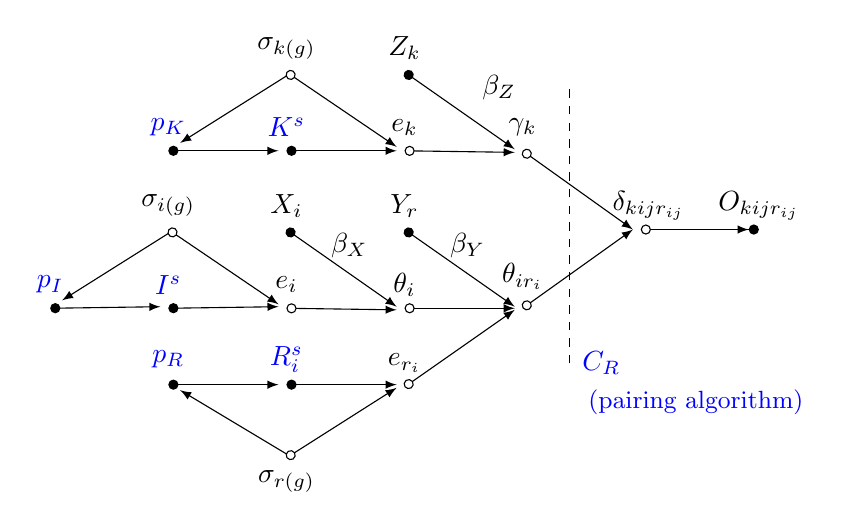
\begin{tikzpicture}

    % main graph
    % nodes (variables)
    \node at (-3,1) {$X_{i}$};
    \node at (-3,0) {$e_{i}$};
    \node at (-1.5,3) {$Z_{k}$};
    \node at (-1.5,2) {$e_{k}$};
    \node at (-1.5,1) {$Y_{r}$};
    \node at (-1.5,0) {$\theta_{i}$};
    \node at (-1.5,-1) {$e_{r_{i}}$};
    \node at (0,2) {$\gamma_{k}$};
    \node at (0,0.1) {$\theta_{ir_{i}}$};
	\node at (1.6,1) {$\delta_{kijr_{ij}}$};
    \node at (3,1) {$O_{kijr_{ij}}$};
    
	% paths
    \draw[{Circle}-{latex}](-3,0.7) to (-1.6,-0.28); % X_i -> theta_i
    \draw[{Circle[open]}-{latex}](-3,-0.3) to (-1.6,-0.32); % e_i -> theta_i
    \draw[{Circle}-{latex}](-1.5,2.7) to (-0.1,1.72); % Z_k -> gamma_k
    \draw[{Circle[open]}-{latex}](-1.5,1.7) to (-0.1,1.68); % e_k -> gamma_k
    \draw[{Circle}-{latex}](-1.5,0.7) to (-0.1,-0.28); % Y_r -> theta_ir
    \draw[{Circle[open]}-{latex}](-1.5,-0.3) to (-0.1,-0.3); % theta_i -> theta_ir
    \draw[{Circle[open]}-{latex}](-1.5,-1.3) to (-0.1,-0.32); % e_ir -> theta_ir
    \draw[{Circle[open]}-{latex}](0,1.7) to (1.4,0.7); % gamma_k -> delta_kijr
    \draw[{Circle[open]}-{latex}](0,-0.3) to (1.4,0.7); % theta_ir -> delta_kijr
    \draw[{Circle[open]}-{latex}{Circle}](1.5,0.7) to (3,0.7); % delta_kijr -> O_kijr

    
	% extras
	% nodes
    \node at (-4.5,0) {\textcolor{blue}{$I^{s}$}}; % population of units
    \node at (-3,2) {\textcolor{blue}{$K^{s}$}}; % population of judges
    \node at (-3,-0.95) {\textcolor{blue}{$R^{s}_{i}$}}; % population of objects
    
    % paths
    \draw[{Circle}-{latex}](-4.5,-0.3) to (-3.1,-0.28); % I -> e_i
    \draw[{Circle}-{latex}](-3,1.7) to (-1.6,1.7); % K -> e_k
    \draw[{Circle}-{latex}](-3,-1.27) to (-1.6,-1.27); % R_i -> e_r(i)


    % node effects
    \node at (-2.2,0.5) {$\beta_{X}$};
    \node at (-0.3,2.5) {$\beta_{Z}$};
    \node at (-0.7,0.5) {$\beta_{Y}$};
    
    \node at (-4.5,1) {$\sigma_{i(g)}$}; 
    \draw[{Circle[open]}-{latex}](-4.5,0.7) to (-3.1,-0.25);
    \draw[-{latex}](-4.5,0.65) to (-5.85,-0.2);

    \node at (-3,3) {$\sigma_{k(g)}$};
    \draw[{Circle[open]}-{latex}](-3,2.7) to (-1.6,1.75); 
    \draw[-{latex}](-3,2.65) to (-4.35,1.8);

    \node at (-3,-2.5) {$\sigma_{r(g)}$};
    \draw[{Circle[open]}-{latex}](-3,-2.2) to (-1.6,-1.31); 
    \draw[-{latex}](-3,-2.15) to (-4.35,-1.34); 

    \node at (-6,0) {\textcolor{blue}{$p_{I}$}}; % population of units
    \node at (-4.5,2) {\textcolor{blue}{$p_{K}$}}; % population of judges
    \node at (-4.5,-0.95) {\textcolor{blue}{$p_{R}$}}; % population of objects

    \draw[{Circle}-{latex}](-6,-0.3) to (-4.6,-0.28);
    \draw[{Circle}-{latex}](-4.5,1.7) to (-3.1,1.7); 
    \draw[{Circle}-{latex}](-4.5,-1.27) to (-3.1,-1.27);
    
    \draw[dashed](0.6,-1) to (0.6,2.5); % straight line
    \node at (1,-1) {\textcolor{blue}{$C_{R}$}};
    \node at (2.2,-1.5) {\textcolor{blue}{\small{(pairing algorithm)}}};

\end{tikzpicture}

\end{document}
